%!TEX root = Projektdokumentation_ClockPendulumAnalyzer.tex
\subsection{Zusammenstellung Hardware und Gehäuse}
\label{cap:housing}
Der vorliegende Abschnitt beschreibt das Zusammenspiel des Sensors mit dem Zähler, die Einstellmöglichkeiten sowie alle Elemente am Gehäuse.
\subsubsection{Anschlüsse und Zusammenbau}
Um Wartungsarbeiten so leicht wie möglich zu gestalten, sind sämtliche Hardware-Elemente steckbar gestaltet. In Abbildung \ref{fig:Anschluesse_hwb} sind die Steckplätze für die einzelnen Anbauteile beschrieben.
\begin{figure}[H]
	\centering
	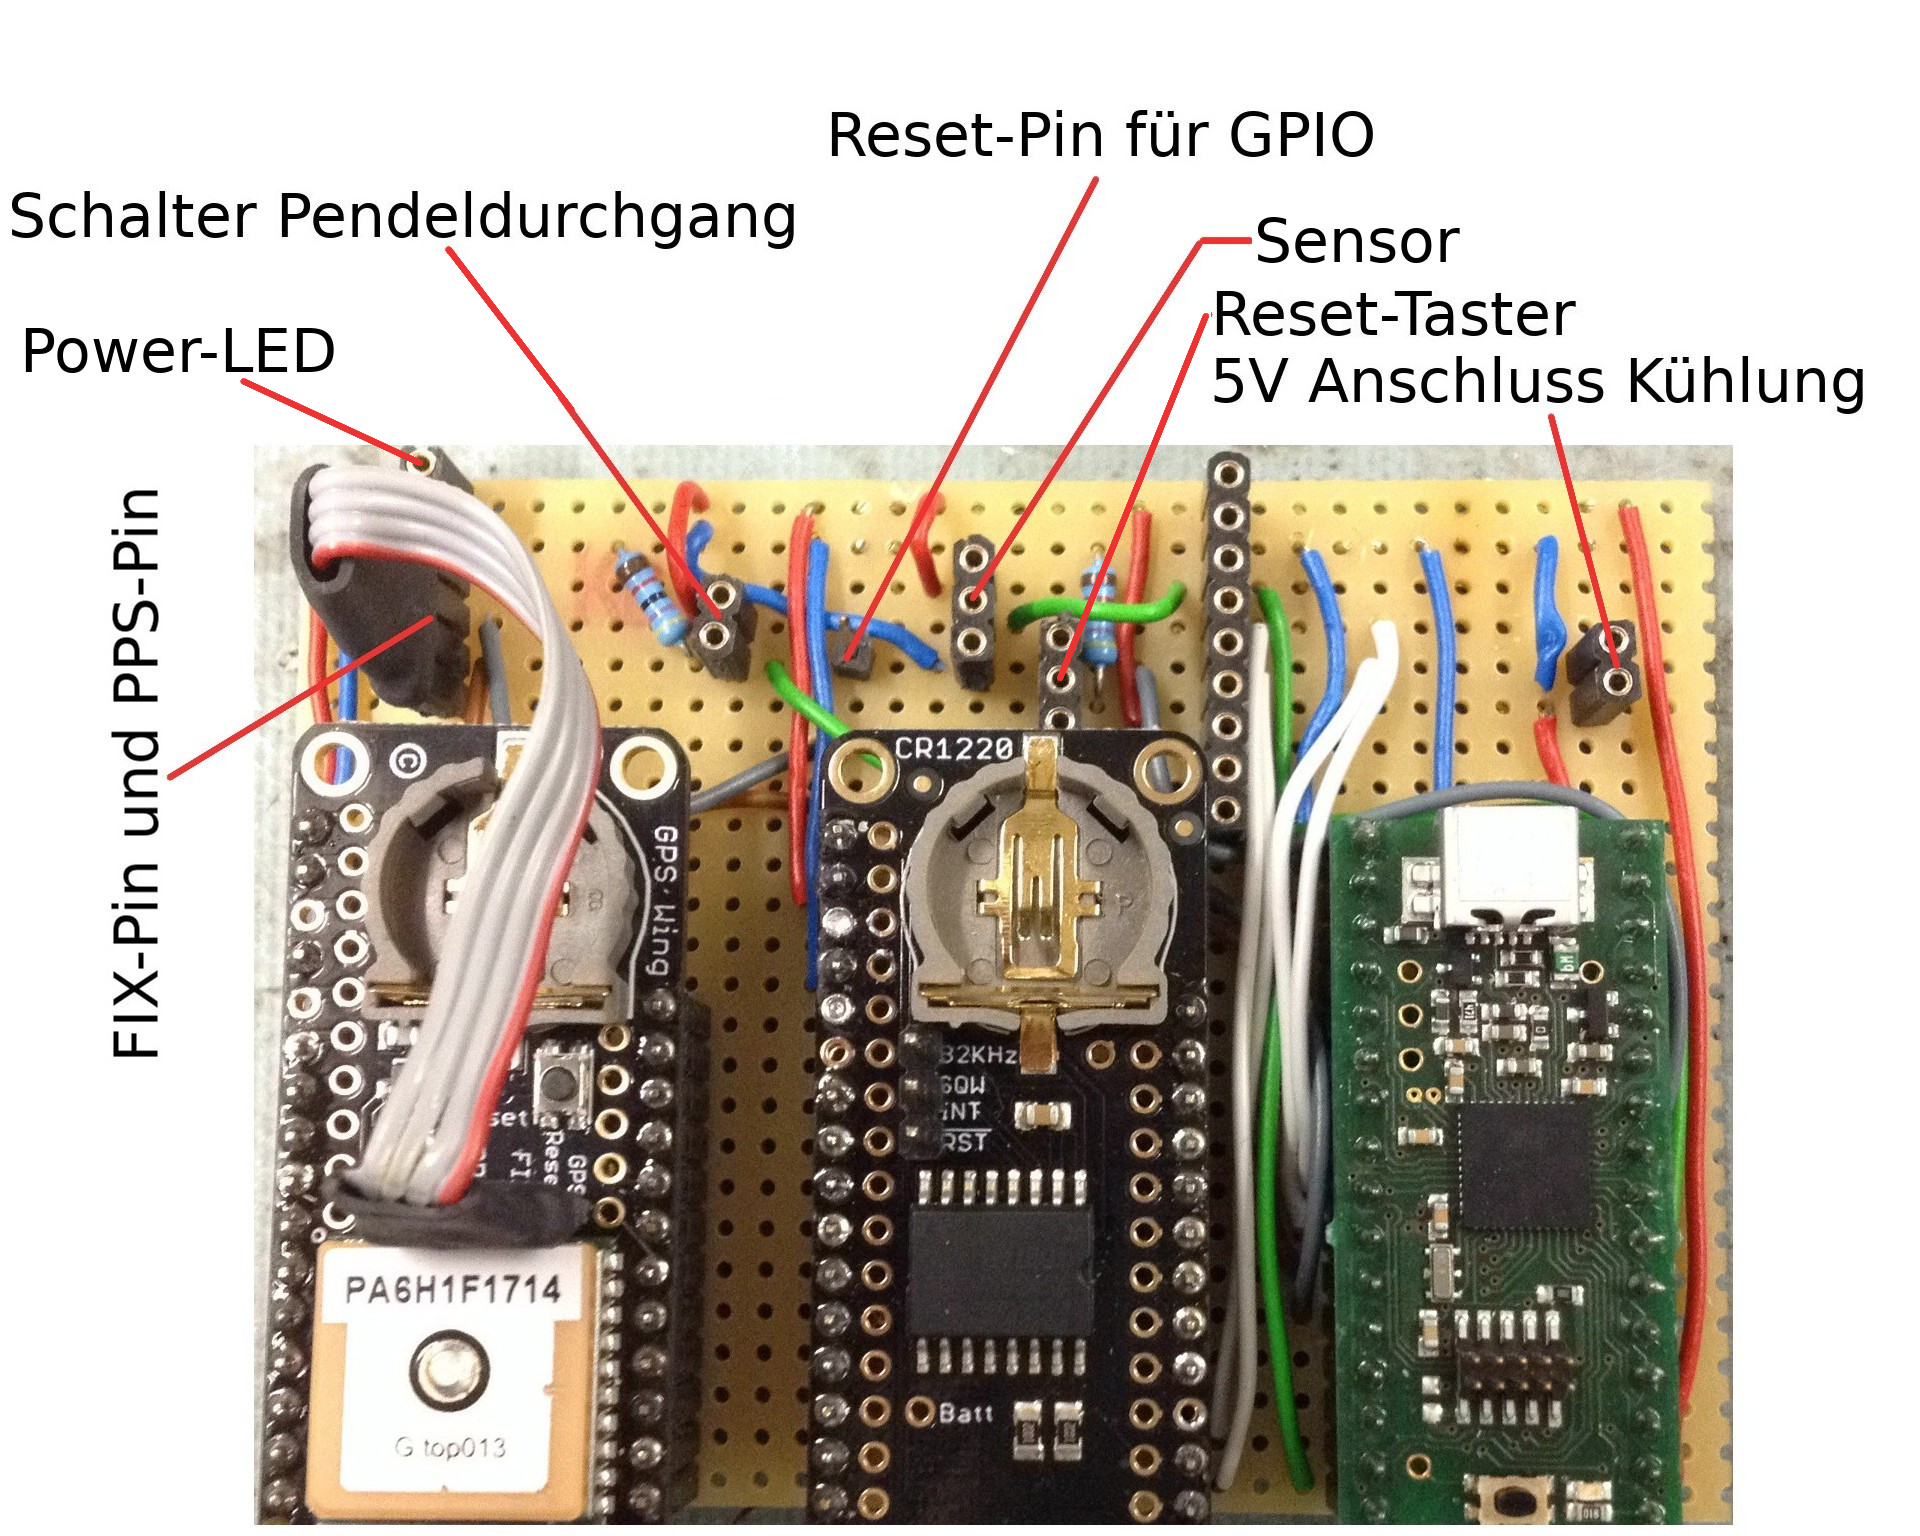
\includegraphics[width=0.5\textwidth]{Anschluesse_hwb}
	\caption{Beschrieb der Anschlüsse auf dem \hwb}
	\label{fig:Anschluesse_hwb}
\end{figure}
\begin{itemize}
	\item Schalter Pendel-Durchgang: Entscheidet, ob jede zweite Messung verworfen wird oder nicht.
	\item Power-LED: Ein, sobald die Stromversorgung besteht.
	\item Reset-Pin für GPIO: Externer Eingang um den Zähler zurückzusetzen.
	\item Reset-Taster: Taster-Anschluss um den Zähler zurückzusetzen.
	\item 5V Anschluss Kühlung: Lüfter-Anschluss.
	\item FIX-Pin und PPS-Pin: Verbindungskabel zum GPS-Modul. Die übrigen zwei Anschlüsse werden nicht weiter verwendet.
\end{itemize}
Das \hwb ist im Gehäuse nicht explizit fixiert, einzig durch zwei Schaumstoffbahnen leicht geklemmt. So kann es leicht entnommen werden, falls Wartungsarbeiten notwendig würden.
\subsubsection{Gehäuse}
Das \rpi und das \hwb befinden sich in einem Sperrholzgehäuse, bei dem die Bodenfläche, der Deckel und zwei Seitenwände mit Kupfer verkleidet sind. 
Die Kupferverkleidung sorgt einerseits für eine gute Wärmeverteilung und bietet einen Schutz vor Funken, sollte ein Bauteil Schaden nehmen.
Zum Schutz vor Feuchtigkeit und Verschmutzung ist die Innenseite des Gehäuses mit einem PU-Lack versehen und die Aussenseite mit Holzöl behandelt. 
Der Deckel schliesst mittels Klemmung und kann mit einem Schraubenzieher oder ähnlichem leicht geöffnet werden.\\
Die Wärme wird mittels dem in Abbildung \ref{fig:housing_side1} sichtbaren Lüfter abtransportiert, was zu konstanten Temperaturverhältnissen im Gehäuse führt.
\begin{figure}[H]
	\centering
	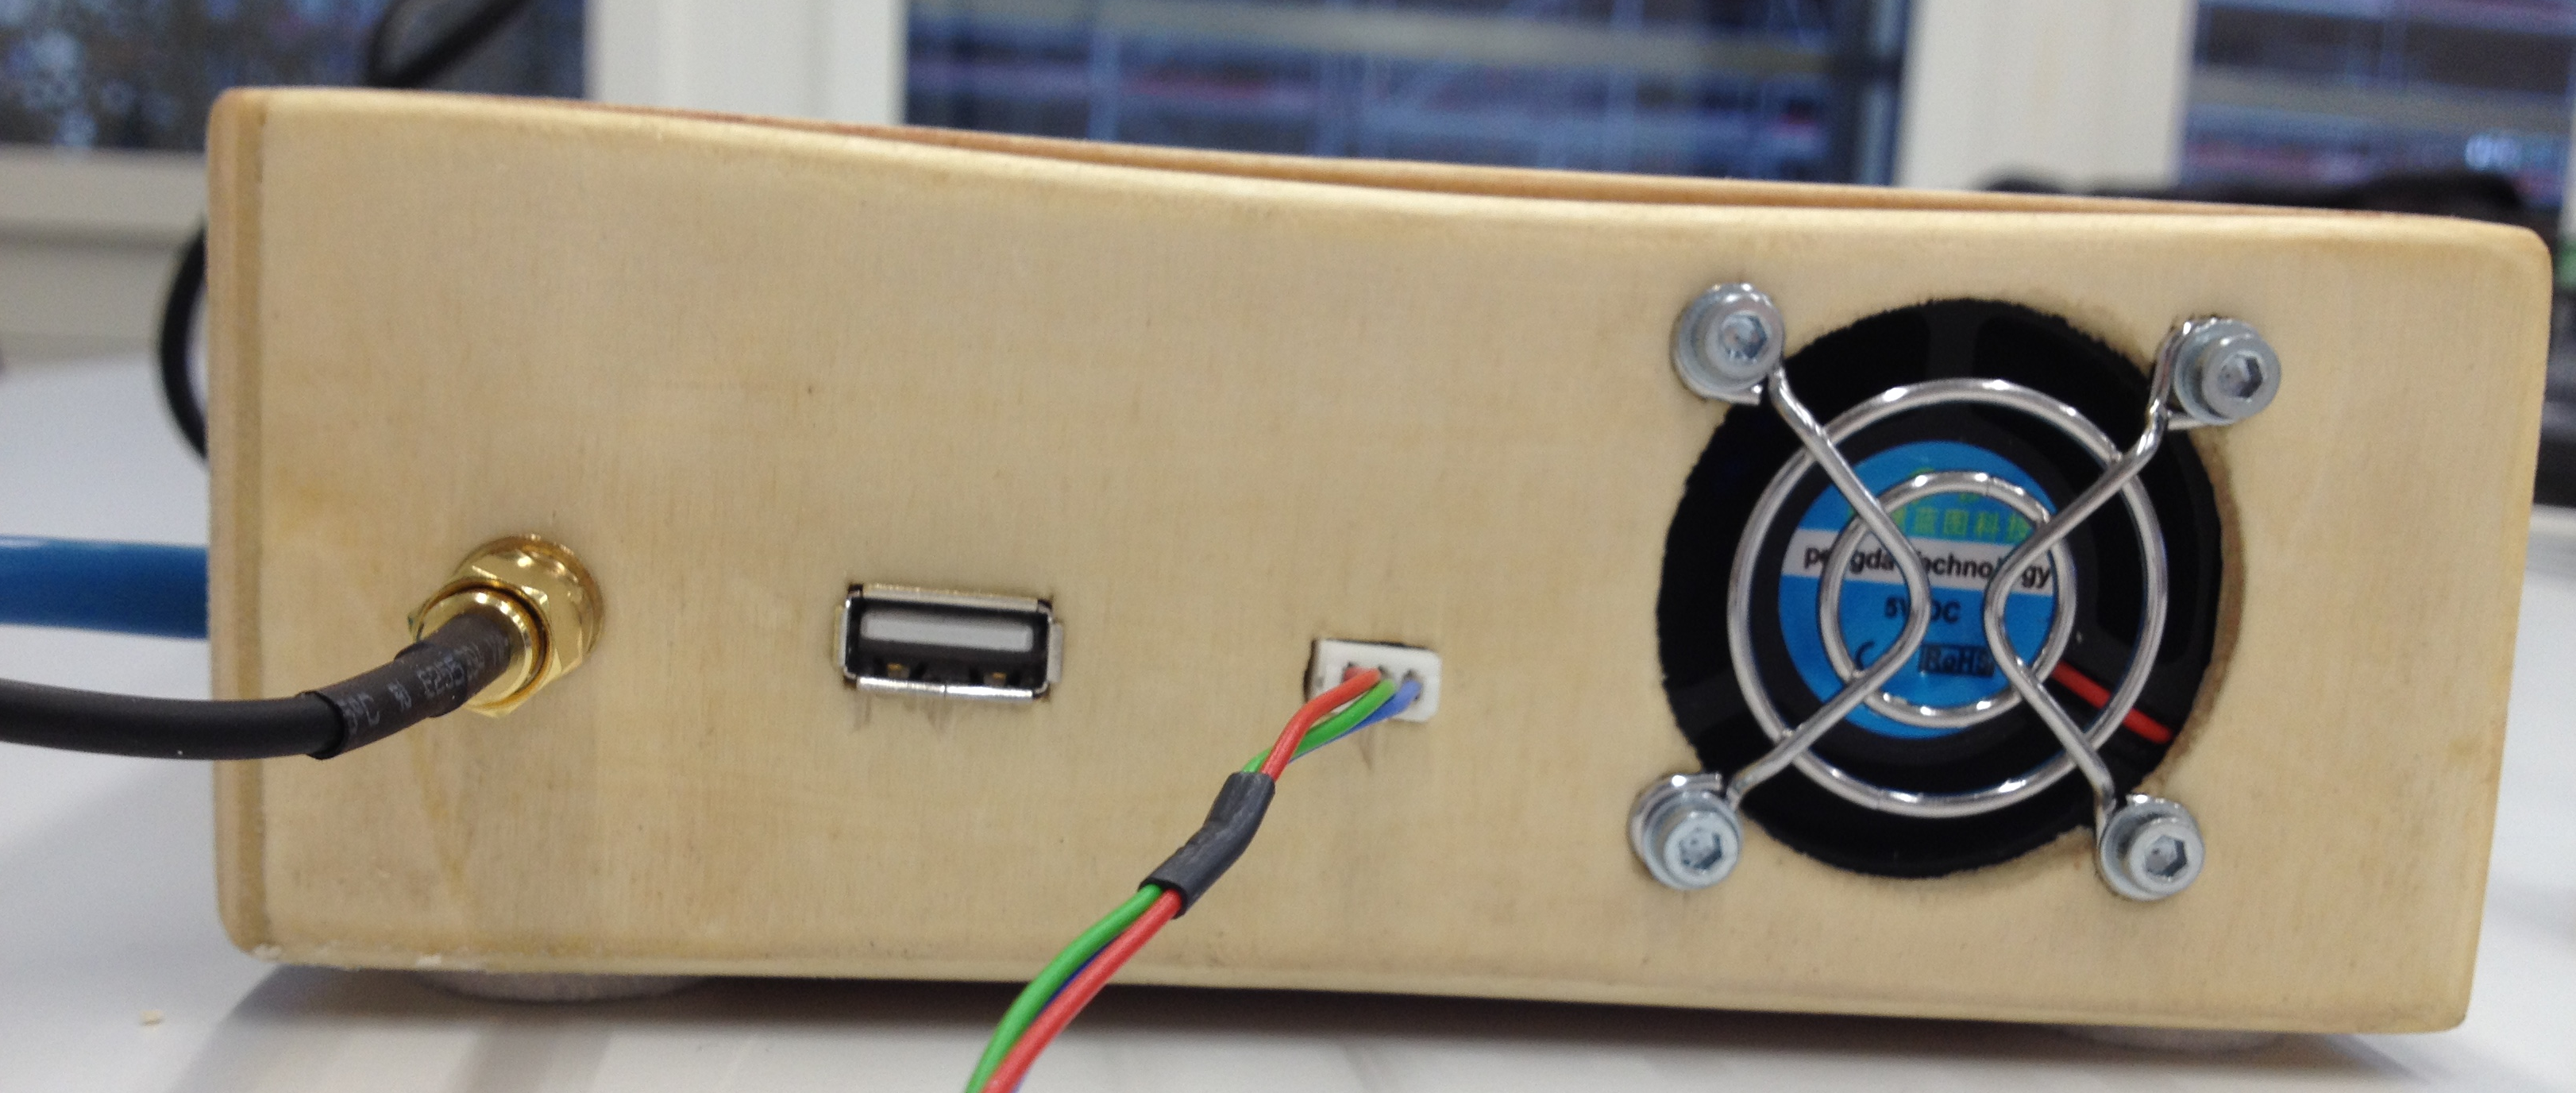
\includegraphics[width=0.5\textwidth]{housing_side1}
	\caption{Lüfterseite des Gehäuses}
	\label{fig:housing_side1}
\end{figure}
\noindent Nebst dem Lüfter befinden sich auf dieser Gehäuseseite der Sensoranschluss, der Anschluss für die GPS-Antenne und ein USB-Port, falls der Datenträger für die Datenbank nicht im Gehäuse Platz finden sollte.\\
Auf der nächsten Gehäuseseite befinden sich der Power-Anschluss des Systems, der HDMI- und der 3.5mm Anschluss des \rpi{}'s und der RJ45 Netzwerkanschluss (Abbildung \ref{fig:housing_side2}).
\begin{figure}[H]
	\centering
	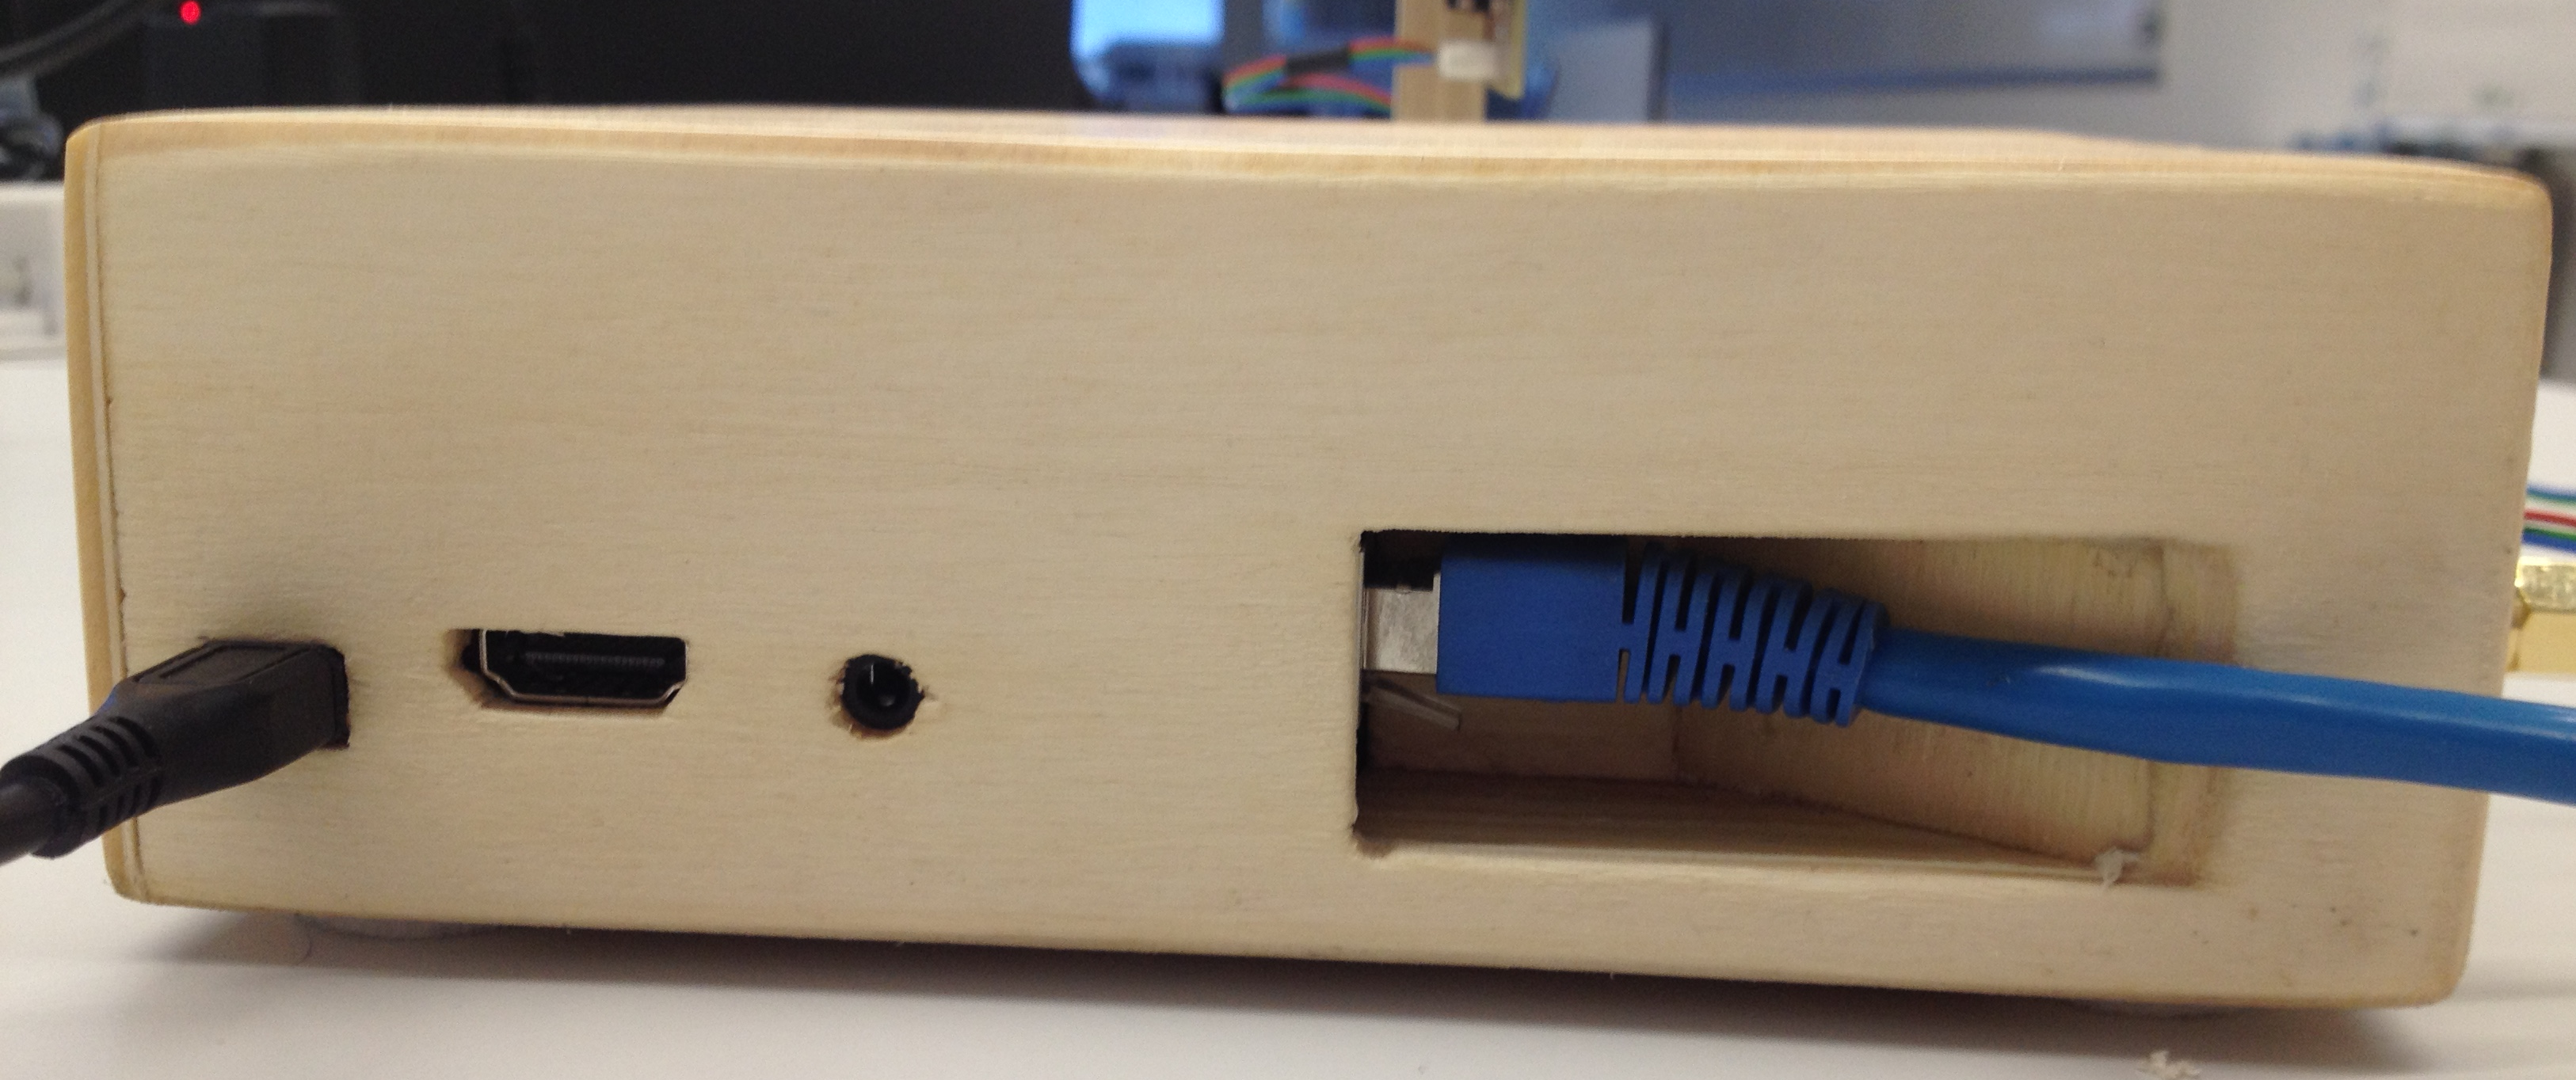
\includegraphics[width=0.5\textwidth]{housing_side2}
	\caption{Anschlusseite für Power und Netzwerk des Gehäuses}
	\label{fig:housing_side2}
\end{figure}
Auf der dritten Seite sind der Reset-Knopf für den Zählerwert (Mitte), der Schalter, ob jede zweite Messung verworfen werden soll und eine Aussparung angebracht, über welche die SD-Karte des \rpi ausgetauscht werden kann (Abbildung \ref{fig:housing_side3}).
\begin{figure}[H]
	\centering
	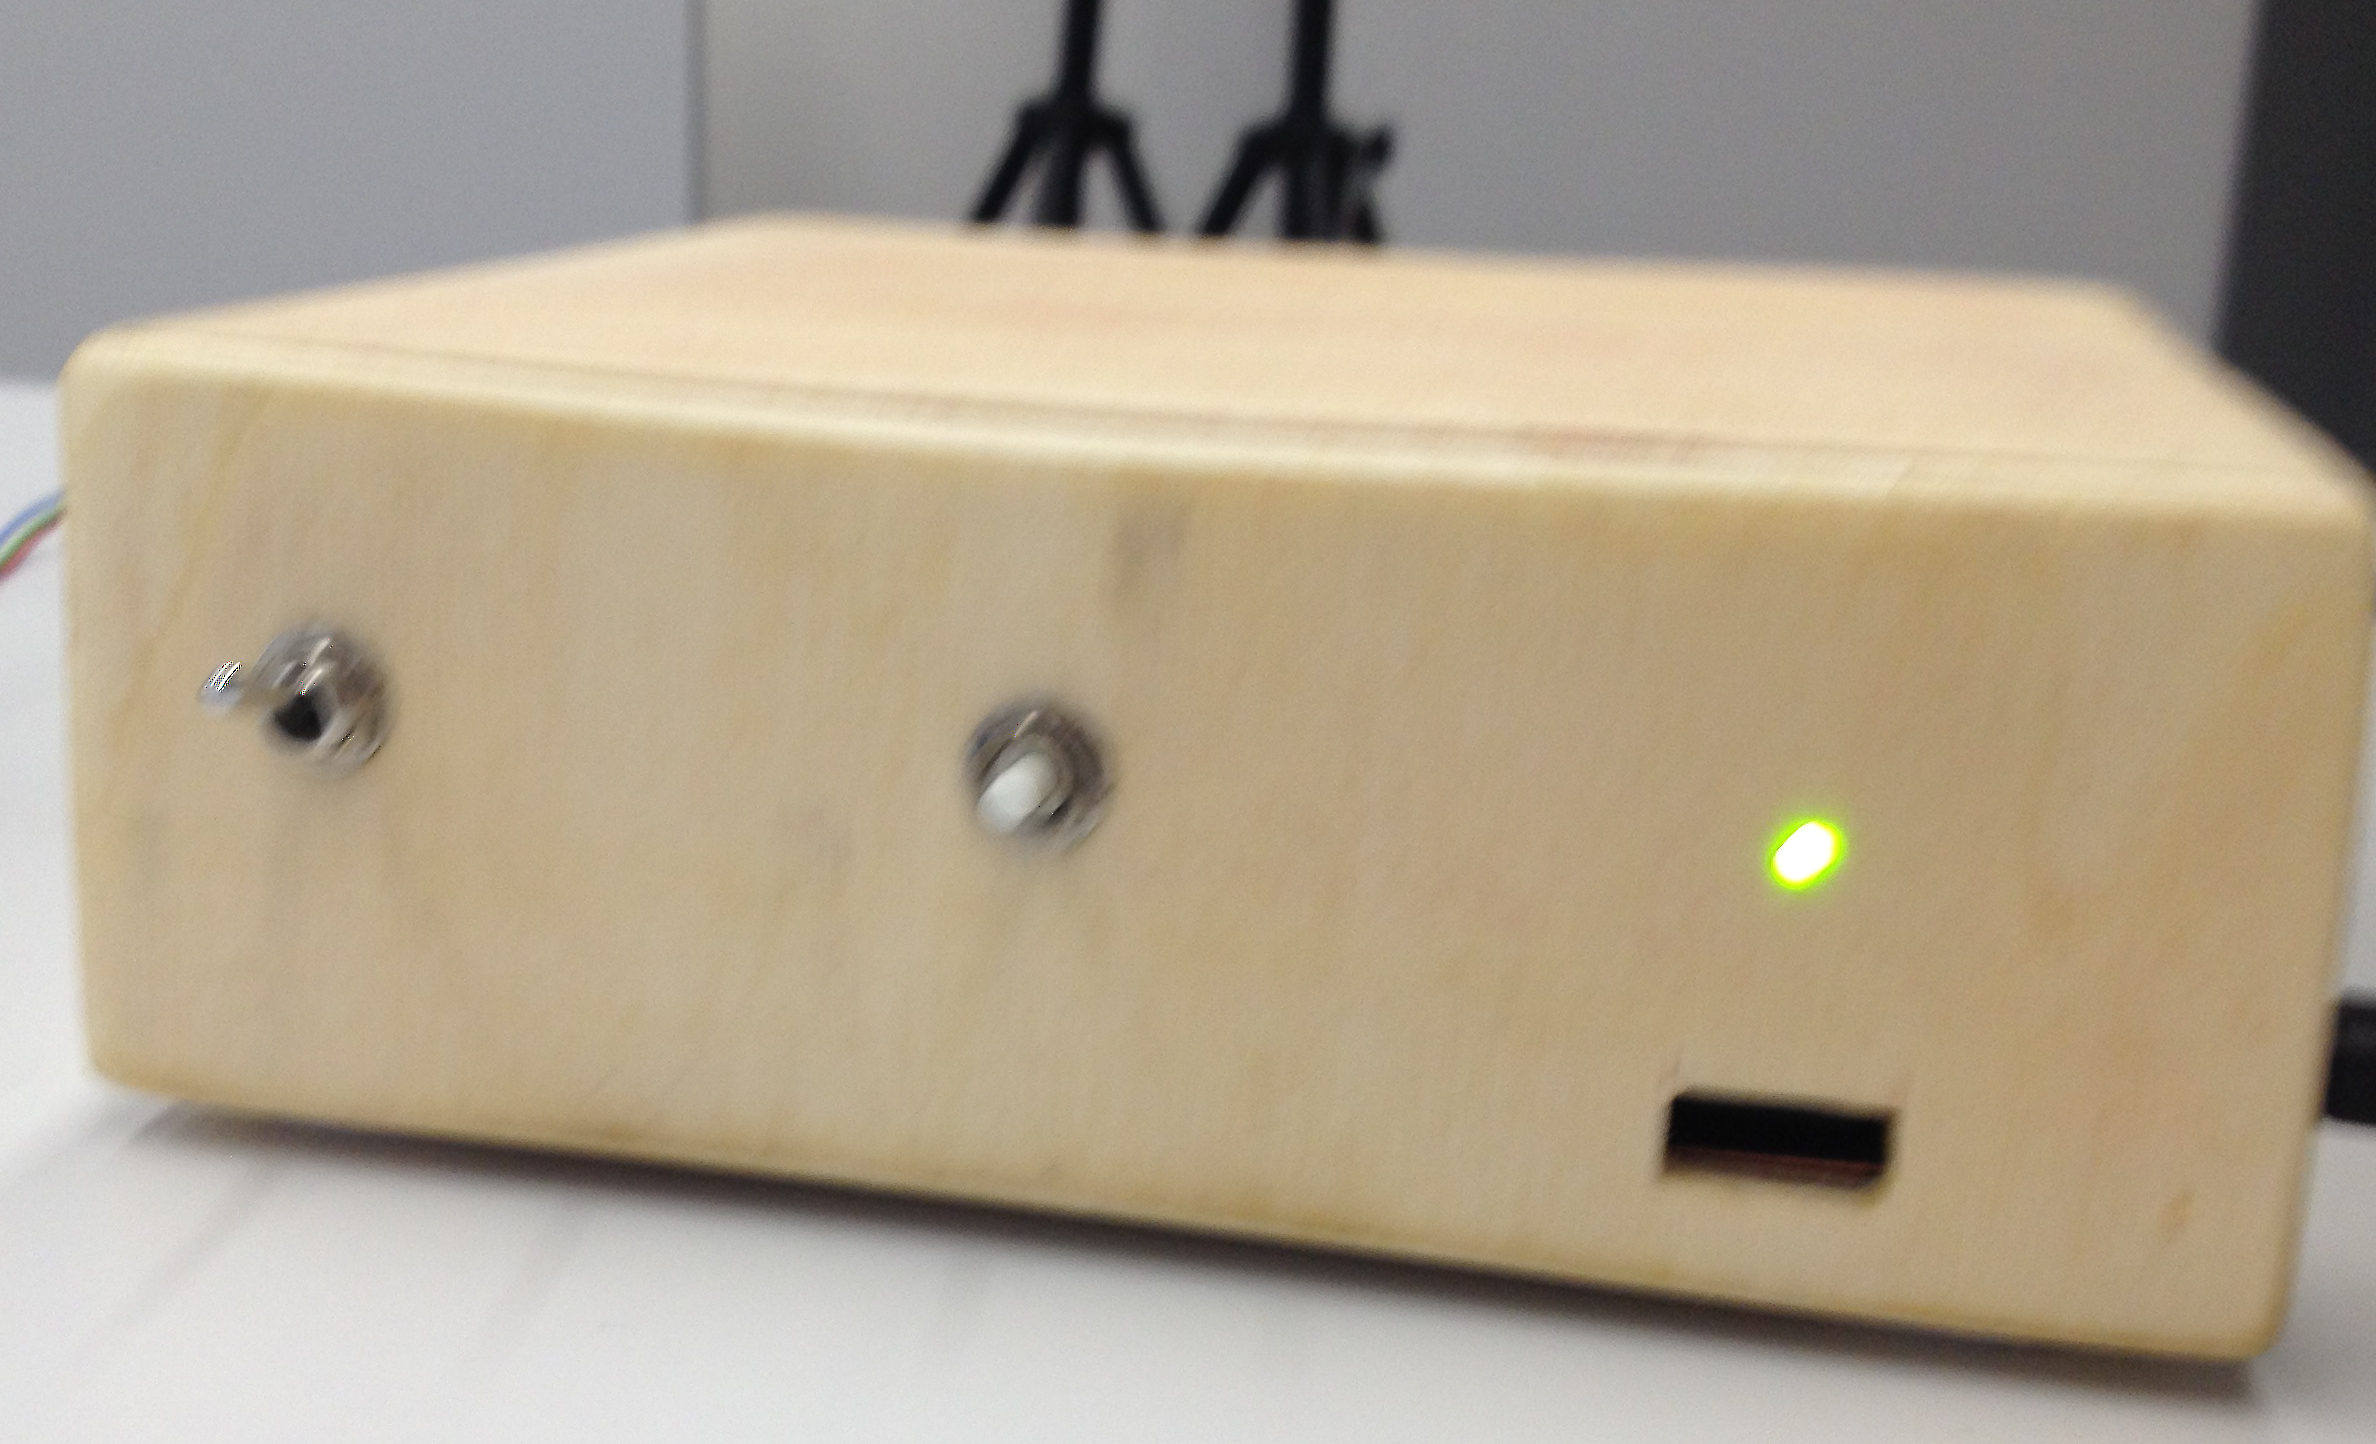
\includegraphics[width=0.5\textwidth]{housing_side3}
	\caption{Gehäuseseite mit Einstell- und Reset-Schalter}
	\label{fig:housing_side3}
\end{figure}